\documentclass[12pt,letterpaper,USenglish]{article}

\usepackage[most]{tcolorbox}
\usepackage{amsmath}
\usepackage{amssymb}
\usepackage{microtype}
\usepackage{tikz}
\usepackage{paralist}
\usetikzlibrary{calc,positioning,backgrounds,intersections,graphdrawing,shapes,graphs,arrows,arrows.meta}
\usegdlibrary{trees}

%%% Please use define.org for macros.
\input{define.orgtex}

\begin{document}

\makeatletter
\tikzset{use path/.code=\tikz@addmode{\pgfsyssoftpath@setcurrentpath#1}}
\makeatother
\tikzset{lead/.style={anchor=north west,font=\it\bfseries,text=algs4red},
    graphs/mytree/.style= {
    tree layout, minimum number of children=2,
    sibling distance=5mm, level distance=5mm,
    nodes={draw, anchor=north,minimum
      height=13pt, fill=white,inner sep=1pt, font=\footnotesize,
      rounded rectangle},
    edges={very thick}},
  graphs/shallowtree/.style={
    mytree,level distance=1mm,sibling distance=15mm,level sep=0},
  algs4arrow/.style={->,>={Latex[length=7pt]},line width=0.8mm,algs4red},
  redlink/.style = {
    algs4red, line width=3pt}}

\noindent\begin{tikzpicture}[every node/.style={anchor=north west}]
  % Main background
  \begin{scope}[on background layer]
    \fill[black!10!white, draw=white, line width=6pt] (-.5\textwidth, 0) rectangle (.5\textwidth, -18cm);
  \end{scope}

  % Clip and left margin
  \path [save path=\theframe, rounded corners] ($(-.5\textwidth, 0) + (1.5pt,-1.5pt)$)
                rectangle ($(.5\textwidth, -18cm) + (-1.5pt, 1.5pt)$);
  \clip [use path=\theframe];
  \coordinate (left) at ($(-.5\textwidth, 0) + (0.3cm,0)$);

  % Title
  \node [anchor=north,text width=20cm,minimum height=1.4cm,align=center,fill=algs4red,text=white]
  {\sffamily\Large \textbf{3.3}\quad BALANCED SEARCH TREES: RED-BLACK TREES};

  % Definition
  \node [lead] (def) at (left |- 0, -1.6cm) {Definition.};
  \node [right=0cm of def.north east, anchor=north west] {%
    \begin{minsizebox}{.8\textwidth}{10cm}
      \begin{compactitem}
      \item A BST that has red and black links, such that red links lean left,
        no node has two red links connected to it, and the tree has perfect
        black balance.\\[0.7em]
      \item Red-black trees are a specific encoding of 2-3 trees.
      \end{compactitem}
    \end{minsizebox}%
  };
  \begin{scope}[xshift=4cm,yshift=-2.6cm]
    \graph[mytree] { r[as={~3~~7~~}] -- {a[as={\(T_1\)},draw=none,fill=none],
        b[as={\(T_2\)},draw=none,fill=none],
        c[as={\(T_3\)},draw=none,fill=none]}};
    \draw[algs4arrow] (1.6cm,-.4cm) -- +(.6cm, 0cm);
    \draw[algs4arrow,<-] (1.3cm,-.4cm) -- +(.6cm, 0cm);
    \graph[shallowtree] {
      7[x=4cm] --[redlink] { 3 -- {a[as={\(T_1\)},draw=none,fill=none],
          b[as={\(T_2\)},draw=none,fill=none]}};
      7 -- {c[as={\(T_3\)},draw=none,fill=none]}};
  \end{scope}
  
  % Example
  \begin{scope}[shift={($(def.south west) + (0cm,-2.3cm)$)}]
    % Background & lead
    \begin{scope}[on background layer]
      \fill[black!15] (-0.07, 0.35) rectangle (19.05, -3.5);
    \end{scope}
    \node[lead,draw=none,shape=rectangle] at (0, 0.3) {Example.};
    \node at (3cm,0cm) {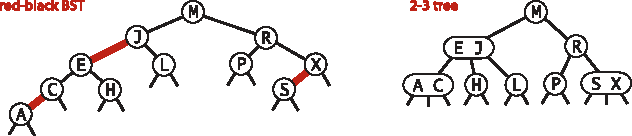
\includegraphics[height=3cm]{rb}};
  \end{scope}
 

  % Rotation, Insertion
  \node [text width=20cm, fill=algs4red,text=white, align=left] (algs) at (-.5\textwidth,-8.5cm)
  {\sffamily\bfseries ~~Rotations, flip, \& insertion};
  \draw[gray,thick] ($(algs.south -| 0, 0) + (1cm,-1cm)$) -- +(0, -2.3cm);

  %% Rotations & flip
  \begin{scope}[shift={($(left |- algs) + (0cm,-.4cm)$)}]
    \node[lead] (s) {Rotations and flips.};
    \node [right=0cm of s.north east,anchor=north west] {Used to restore being a
      red-black tree, preserve black balance and being a BST.};
    
    \begin{scope}[shift={(2.5cm,-1.3cm)}]
      \graph[shallowtree] { 7 --[redlink] { 3 --
          {a[as={\(T_1\)},draw=none,fill=none],
            b[as={\(T_2\)},draw=none,fill=none]}}; 7 --
        {c[as={\(T_3\)},draw=none,fill=none]}};

      \graph[shallowtree] { 3[x=5cm] --
        {c[as={\(T_1\)},draw=none,fill=none]}; 3 --[redlink] { 7 --
          {a[as={\(T_2\)},draw=none,fill=none],
            b[as={\(T_3\)},draw=none,fill=none]}}};

      \node[font=\footnotesize,text width=2cm,align=center] (p) at (1.5cm, 0) {right
        rotation\\
        ~\\
        left rotation};
      \draw[algs4arrow] ($(p.center)+(-.3cm,0.1cm)$) -- +(.8cm, 0cm);
      \draw[algs4arrow] ($(p.center)+(.3cm,-0.15cm)$) -- +(-.8cm, 0cm);
    \end{scope}

    \begin{scope}[shift={(12.7cm,-0.7cm)}]
      \graph[shallowtree,minimum number of children=1,
      sibling distance=7mm,sibling sep=0] {
        f[as=,draw=none,fill=none] -- {
          5[level pre sep=0.2cm] --[redlink] {3 -- {t1 [as={\(T_1\)},draw=none,fill=none],
                             t2 [as={\(T_2\)},draw=none,fill=none]},
                        8 -- {t3 [as={\(T_3\)},draw=none,fill=none],
                          t4 [as={\(T_4\)},draw=none,fill=none]}}}};

      \graph[shallowtree,minimum number of children=1,
      sibling distance=7mm,sibling sep=0] {
        f[x=4cm,as=,draw=none,fill=none] --[redlink] {
          5[level pre sep=0.2cm] -- {3 -- {t1 [as={\(T_1\)},draw=none,fill=none],
                             t2 [as={\(T_2\)},draw=none,fill=none]},
                        8 -- {t3 [as={\(T_3\)},draw=none,fill=none],
                          t4 [as={\(T_4\)},draw=none,fill=none]}}}};
      \node[font=\footnotesize,text width=2cm,align=center] (p) at (1cm, -0.5cm)
      {flip};
      \draw[algs4arrow] ($(p.center)+(-.4cm,--0.3cm)$) -- +(.8cm, 0cm);
    \end{scope}
  \end{scope}
  
  %% Insert
  \begin{scope}[shift={($(left |- algs) + (0cm,-3.8cm)$)}]
    \node[lead] (s) {Insert.};
    \node [right=0cm of s.north east,anchor=north west] {Insert at leaf with
      red link, then restore being a red-black tree, bottom up.};
    \node at (4cm,-.8cm) {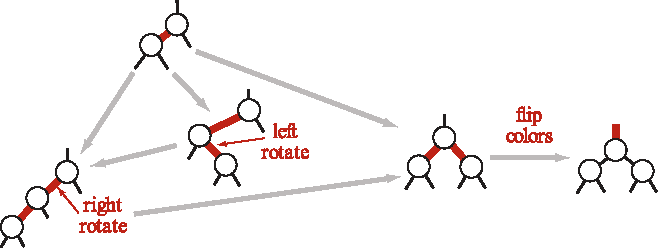
\includegraphics[height=4cm]{insrb}};
  \end{scope}
  

  %% Box
  \draw [algs4red,line width=3pt] [use path=\theframe];

\end{tikzpicture}
\end{document}
%%% Local Variables:
%%% ispell-local-dictionary: "en_US"
%%% TeX-master: t
%%% End:
